

\pagestyle{empty}

\begin{titlepage}
\vspace*{\fill}
\begin{center}
\begin{picture}(300,510)
  \put( 10,520){\makebox(0,0)[l]{\large \bf \textsc{Department of Fundamental Problems of Technology}}}
  \put( 10,500){\makebox(0,0)[l]{\large \bf \textsc{Wroclaw University of Technology}}}
  \put( 0,330){\makebox(0,0)[l]{\huge \bf \textsc{Electronic Prescriptions System}}} 
  \put( 0,305){\makebox(0,0)[l]{\huge \bf \textsc{Database \& Server Documentation}}}
  \put(145,240){\makebox(0,0)[l]{\large     \textsc{Michal Kaczmarek}}}
  \put(145,220){\makebox(0,0)[l]{\large     \textsc{Pawel Kedzia}}}
  \put(145,200){\makebox(0,0)[l]{\large     \textsc{Jakub Plaskonka}}}
  \put(145,180){\makebox(0,0)[l]{\large     \textsc{Mateusz Platek}}}

  \put(100,-80){\makebox(0,0)[bl]{\large \bf \textsc{Wroclaw 2014}}}
\end{picture}
\end{center}
\vspace*{\fill}
\end{titlepage}

\newpage

\pagestyle{headings}

\section{Introduction}

\subsection{Current situation}

Current system strongly depends on paper prescriptions. Each prescriptions carries a lot of data, which some can be treated as private data of patients:
\\
\begin{itemize}
	\item prescription's creation date,\\
	\item patient's personal data:\\
	\begin{itemize}
		\item name and surname
		\item address
		\item PESEL\\
	\end{itemize}
	\item number of the prescription, specific for each doctor \footnote{NFZ generates the list of the prescription for the specific doctor. Every prescription have the unique
	identifier number. While the refund process, the NFZ checks, if the number on the prescription, the
	doctor name, signature and stamp are correct. Only if there are valid, the refund is given back.},\\
	\item list of medicines with level level of refund,\\
	\item signature and stamp of the doctor.\\
\end{itemize}

The patient, who was given the prescription by the doctor, goes to the pharmacy to buy the medicines. He gives his prescription to a pharmacist and says which of the medicines from the list he wants to buy. The pharmacist checks if the medicines are available and if yes, he sells them. Next, he takes the prescription and makes a signature next to the each of the medicine he sold. He also inputs to the software installed on
computers in the pharmacy, which of the medicine was sold, for who, who gave the prescription and what are the costs of the refund.\\

Each month in every pharmacy a report, consisting of the set of the information about each prescription sold in the pharmacy is generated. This report is sent to the NFZ central database. Based on this, the NFZ refunds costs of the medicines. Each prescription has to be kept for at least five years in the pharmacy, and be ready for checking during controls made by NFZ representatives.
\clearpage
%\begin{figure}[h]
%	\centering
%	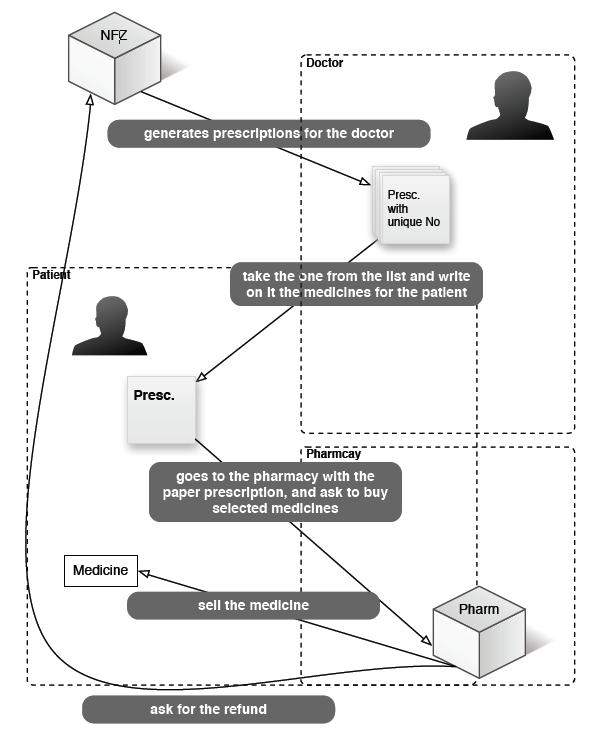
\includegraphics[width=0.9\textwidth]{database/current_uml.png}
%	\caption{The main points of currently used system}
%	\label{fig:F1}
%\end{figure}


\subsection{Threats and Inconveniences}
The way prescriptions are currently processed is vulnerable to many threats, and brings many inconveniences. The most important ones are listed below.

\begin{longtable}{|p{3cm}|p{9cm}|}
    
    \hline
    \centering Party & Threats and Inconveniences \\ \hline
    \vspace*{\fill} \begin{quote} \centering Patient \end{quote} \vspace*{\fill} & \begin{itemize}
    \item the patient can lose the prescription and he cannot
    buy the medicines, even if they are lifesaving,
    he has to go to the doctor again and ask
    for the new prescription \newline
    \item the patient can lose his prescription, then, the
    person who found this prescription can buy this
    medicines; what is more, this person can get to
    know, who takes which medicines and in this
    way, he can get to know, what is wrong with
    the person described on the prescription
    
    \end{itemize}
    \\ \hline
  
    \hline
    \vspace*{\fill} \begin{quote} \centering Doctor  \end{quote} \vspace*{\fill} & \begin{itemize}
    \item Doctor can create prescriptions without knowledge of patient and use them in fraud proccess.
    Doctor can work with pharmacy and drugs producer to get money from NFZ refundations without selling any actual drugs.
    pharmacies \newline
    \item Doctors which see the patient for the first time not always have access to the disease or drugs history.

    \end{itemize}
    \\ \hline

     \hline
     \vspace*{\fill} \begin{quote} \centering Pharmacy \end{quote} \vspace*{\fill} & \begin{itemize}
     \item the pharmacy has to wait long time to refund
     costs for the medicines from NFZ on \newline
     \item the prescription are often mistakes, which make
     the prescription useless. In this situation, the
     patient has to go to the doctor again and ask
     him to fix the mistakes
     \end{itemize}
     \\ \hline


  \hline
  \vspace*{\fill} \begin{quote} \centering NFZ \end{quote} \vspace*{\fill} & \begin{itemize}
  \item significant amount of money is being defrauded
  from NFZ, because the current system does not
  verify if the patient himself has bought the
  medicine or the pharmacists has made a false
  call for the medicine having some patient?s prescription,
  prepared by the doctor (who is also a
  part of the defraudation scheme)
  \end{itemize}
  \\ \hline


    \hline
    \vspace*{\fill} \begin{quote} \centering System  \end{quote} \vspace*{\fill} & \begin{itemize}
    \item the patient can try to copy the prescription and
    try to buy the medicines few times in different
    pharmacies \newline
    \item the patient can claim that he has lost his prescription
    and ask the doctor to give him another
    one, then, he can buy the medicines twice instead
    of once
    \end{itemize}
    \\ \hline

\end{longtable}

\subsection{Systems goal}

The system has to eliminate each of the flaws described in previous subsection.
It will meet each of following requirements:
\begin{itemize}
\item Prescriptions will be digitalized .
\item Prescriptions will be hard to forge.
\item Doctors won't be able to create prescriptions without knowledge of patient.
\item Prescriptions will be realized only by users with right credentials.
\item Patients and doctors will be able to browse history of prescriptions.
\item System will be secured with most up-to-date measures.
\item System will provide anonymous big data statistics.
\end{itemize}

\subsection{Central Server tasks}

The central server will be the core component of the whole digital prescriptions system. Key features of central server are:
\begin{itemize}
 \item Holding data of patients, doctors and pharmacists
 \item Allowing doctors to create prescriptions
 \item Allowing doctors and patients to review history of created prescriptions
 \item Allowing patients to transfer the ownership of prescription in secure, controlable manner
 \item Allowing pharmacists to review prescriptions yet to be realized
 \item Allowing prescription realization only if patient will be present at this event
 \item Validating the signatures of each party
 \item Providing annonymous statistics
\end{itemize}

\newpage
\section{Use cases}
We define two groups of actors - clients like patients, doctors and pharmacists which benefit from the system on daily basis and third parties - administrators, analytic tools and goverment authorities which cope with the system on special ocassions.

\begin{figure}[h]
\centering
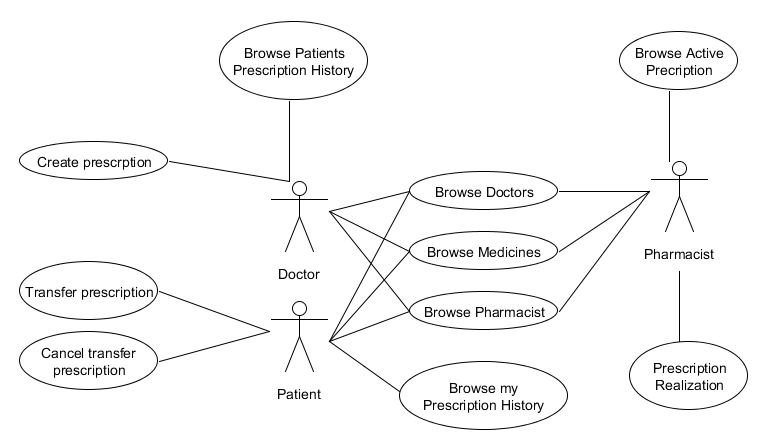
\includegraphics[width=1\textwidth]{database/standardUseCases.png}
\end{figure} 
\textbf{ We only describe use cases from DB point of view.
Detailed description of client side use cases should be found in their respective specifications.}

Every use case requires the users to establish secure channel of communication with central server and have to be logged in which will be described more thorougly in section~\ref{sec:login}.
\subsection{Shared use cases}

Three use cases are applicable for patient, pharmacist and doctors and they consider browsing informations which can be publicly accessible, that is:
\begin{itemize}
\item Browse Doctors
\item Browse Medicines 
\item Browse Pharmacists
\end{itemize}
Rest of use cases which are applicable to only one actor is described in their respective subsections.

\begin{longtable}{|p{6cm}|p{7.75cm}|}
   
    \hline
    Actors: Patient, Doctor, Pharmacist &Title: Browse Doctors \\ \hline
    Goal: & Allows to find doctor with specific name, address or license number. \\ \hline
    Scenario: & User enters any or all of name, address and license number of searched doctor. \\ \hline
    Result: & List of doctors corresponding to the query. \\ \hline
    Database  method: & browse\_doctors \\ \hline
    
\end{longtable}

\begin{longtable}{|p{6cm}|p{7.75cm}|}
    
    \hline
    Actors: Patient, Doctor, Pharmacist &Title: Browse Pharmacies \\ \hline
    Goal: & Allows to find pharmacist and pharmacy with specific name, address or license number. \\ \hline
    Scenario: & User enters any or all of name, address, license number of searched pharmacist or pharmacy name. \\ \hline
    Result: & List of pharmacists corresponding to the query. \\ \hline
    Database  method: & browse\_pharmacies \\ \hline

\end{longtable}


    \begin{longtable}{| p{6cm} | p{7.75cm} |}
    \hline
    Actors: Patient, Doctor, Pharmacist &Title: Browse Medicines \\ \hline
    Goal: & Allows to find medicine with specific name or type. \\ \hline
    Scenario: & User enters name or/and type of medicine he is searching. \\ \hline
    Result: & List of medicines corresponding to the query. \\ \hline
    Database  method: & browse\_medicines \\ \hline
    \end{longtable}


\subsection{Patient use cases}


    \begin{longtable}{| p{6cm} | p{7.75cm} |}
    \hline
    Actors: Patient &Title: Transfer prescription \\ \hline
    Goal: & Allows to transfer a prescription to another patient and give him credentials to realize this prescription. Patient who transferred the prescription losses his right to realize it by himself. If he wants the prescription back he has to cancel the transfer (next use case). \\ \hline
    Scenario: & Patient enters his id, id of new owner, the prescription id he wants to transfer and his signature. \\ \hline
    Result: & OK response from database and iId of new owner of prescription. \\ \hline
    Database  method: & transfer\_prescription \\ \hline
\end{longtable}

    \begin{longtable}{| p{6cm} | p{7.75cm} |}
    \hline
    Actors: Patient &Title: Cancel Transfer Prescription \\ \hline
    Goal: & Allows to revert transfering of prescription to another patient. \\ \hline
    Scenario: & Patient enters his id, prescription id he wants transfers to revert and his signature. \\ \hline
    Result: & OK response from database. \\ \hline
    Database  method: & cancel\_prescription\_transfer \\ \hline
\end{longtable}

    \begin{longtable}{| p{6cm} | p{7.75cm} |}
    \hline
    Actors: Patient &Title: Browse My Prescriptions History \\ \hline
    Goal: & Patient can see his history of realized and created prescriptions.\\ \hline
    Scenario: & Patient sends his id which is signed by his key from smartcard. Patient can define the time span of returned prescriptions as also a filter to only return prescriptions which aren't realized yet. \\ \hline
    Result: & List of prescriptions for the patient. \\ \hline
    Database  method: & browse\_prescription\_history \\ \hline

\end{longtable}

\subsection{Doctors use cases}


    \begin{longtable}{| p{6cm} | p{7.75cm} |}
    \hline
   Actors:  Doctor &Title: Create prescription \\ \hline
    Goal: & Allows to create a new prescription in database for selected patient..\\ \hline
    Scenario: & Doctor enters his and patients ids, as well as the data specific to the medicine - id, dosage, unit and quanitity. Everything is signed by his key. \\ \hline
    Result: & OK response from database. \\ \hline
    Database  method: & create\_prescription \\ \hline
    \end{longtable}



    \begin{longtable}{| p{6cm} | p{7.75cm} |}
    \hline
    Actors: Doctor &Title: Browse Patients Prescriptions History \\ \hline
    Goal: & Doctor can see patient history of realized and created prescriptions..\\ \hline
    Scenario: & Doctor sends his id - he will see all prescriptions created by him. If he will add the id of patient with patients signature, he will see the full history of prescriptions of current patient. Doctor can define the time span of returned prescriptions as also a filter to only return prescriptions which aren't realized yet. \\ \hline
    Result: & List of prescriptions for the patient. \\ \hline
    Database  method: & browse\_patient\_prescription\_history \\ \hline
    \end{longtable}


\subsection{Pharmacist use cases}


    \begin{longtable}{| p{6cm} | p{7.75cm} |}
    \hline
    Actors: Pharmacist &Title: Prescription realization\\ \hline
    Goal: & Pharmacist realizes the prescription. DB checks if the request can be verified and if the prescription is valid.\\ \hline
    Scenario: & Pharmacist enters his id, prescription id as well as drugs id, dosage and qunatity of medicine. Everything is signed by pharmacist key. \\ \hline
    Result: & OK response from database if operation was successful. \\ \hline
    Database  method: & prescription\_realization \\ \hline
    \end{longtable}



    \begin{longtable}{| p{6cm} | p{7.75cm} |}
    \hline
    Actors: Pharmacist &Title: Browse Active Prescriptions \\ \hline
    Goal: & Pharmacist can see prescriptions which are not yet realized. \\ \hline
    Scenario: & Pharmacist sends his id and id of current patient which are signed by both of their keys. Pharmacist can see only prescriptions which are not yet realized. \\ \hline
    Result: & List of prescriptions for the patient. \\ \hline
    Database  method: & browse\_active\_prescriptions \\ \hline
    \end{longtable}


\subsection{Special users use cases}

There are also defined three other users which cope with the system on special ocassions.
These are - administrator, which maintains the system, analytic tools which can be used to obtain statistical data and the goverment authority which has super access to all the data after acquiring proper permissions from court or police.

\begin{figure}[h]
\begin{center}
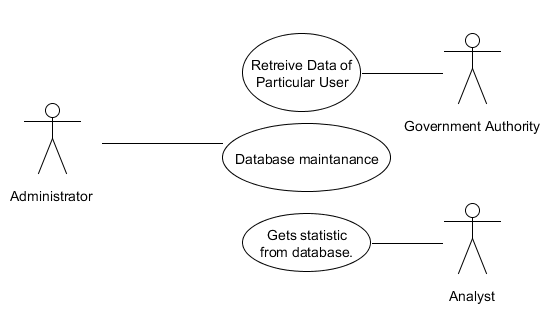
\includegraphics[width=1\textwidth]{database/specialUseCases.png}
\end{center}
\end{figure} 


    \begin{longtable}{| p{6cm} | p{7.75cm} |}
    \hline
    Actor: Administrator &Title: Central Server maintenance \\ \hline
    Goal: & Administrator modifies the database, upgrades software etc. \\ \hline
    \end{longtable}



    \begin{longtable}{| p{6cm} | p{7.75cm} |}
    \hline
    Actor: Goverment Authority &Title: Retreive Data Of Particular User \\ \hline
    Goal: & Goverment Authority (GA) can retreive all sensitive data of every user after showing permission to do so e.g. court order. GA account password can be separated into several pieces to ensure that one attacker won't be in possesion of the key. \\ \hline
    \end{longtable}



    \begin{longtable}{| p{6cm} | p{7.75cm} |}
    \hline
    Actor: Analytic tools &Title: Obtaining statistics from DB \\ \hline
    Goal: & Analyst can query the database for statistical data e.g. number of medicines sold in last month. Analyst can't query patients or link prescriptions data to particular person. \\ \hline
    \end{longtable}


\section{Central Server Architecture}

Central server will be constructed of several components. In order to provide all necessary data and functionalities to the users this is system will be a cooperation of system's logic, specific APIs and database. Now we will provide for auditor what tools will be used in process of system creation
\begin{itemize}
\item Server layer - Apache HTTP Server ("Apache") version 2.4.9
\item Database layer - PostgreSQL version 9.3
\end{itemize}

\subsection{Sequence diagrams for use cases}
\begin{figure}[h]
\centering
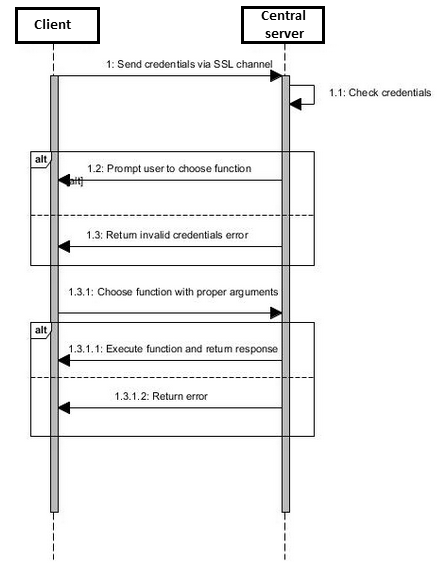
\includegraphics[width=0.7\textwidth]{database/sequence.png}
\caption{General communication diagram for patient, pharmacist and doctor}
\end{figure} 
Every communication with database can be described by one abstract scenario.
First central server and client establish session via SSL. After correct establishment of session, client chooses one of database functions that he can execute with appropriate arguments. Before using methods requiring signatures, client has to ask server for nonce, generated specially for the user. After obtaining the nonce, client can execute selected function.
Database verifies the correctness of signature and data passed in arguments and returns the result, or if one of the verification steps failed, error message.


\subsection{Two-Way SSL}

Two-Way SSL provides the same functionalities as SSL, with the addition of authentication and non-repudiation of the client authentication, using digital signatures. When mutual authentication is used the server would request the client to provide a certificate in addition to the server certificate issued to the client.
The main advantages of client-certificate authentication are:
\begin{itemize}
\item The private information (the private key) is never sent to the server. The client doesn't let its secret out at all during the authentication.
\item A server that doesn't know a user with that certificate can still authenticate that user, provided it trusts the CA (Certificate Authority) that issued the certificate (and that the certificate is valid). This is very similar to the way passports are used: you may have never met a person showing you a passport, but because you trust the issuing authority, you're able to link the identity to the person.
\end{itemize}

\subsubsection{Issuing certificates}
In Two-Way SSL both parties (client and server) need the certificates. The certificate is issued by trusted CA based on public key provided by the party. CA can also generate a keypair for the client or server. It is CA's resposibility to validate identity of party for which it will generate a certificate. Simplest method of such validation would require a CA's official to verify party's identity in person, by checking ID.

Keys used for connecting and authorising should have sufficient length to provide security. If the RSA key is used it should have length of at least 2048 bits. 

\subsection{Connecting to Central Server}\label{sec:login}
\begin{enumerate}
\item Enter smartcard with users private key and certificate (or establish paths to them)
\item set path of PostgreSQL to environment variable PATH.

\item in command line write $psql$ $'host=hosts_ip$ $port=port\_address$ $dbname=database\_name$ $user=username$ $sslmode=require$ $sslcert=user.crt$ $sslkey=user.key$ $sslrootcert=ca.crt'$ where:
	\begin{itemize}
	\item $host$ - IP of server where database is
	\item $dbname$ - is the name of database to which we want to connect
	\item $user$ - name of user which want to connect. Each part will have its own user name.
	\item $sslcert$ - certificate of user.
	\item $sslkey$ - private key of user.
	\item $sslrootcert$ - Certificate of CA.
	\end{itemize}
	Example login: $psql$ $'host=95.85.28.156$ $port=5432$ $dbname=PrescriptionSystem$ $user=patient$ $sslmode=require$ $sslcert=patient.crt$ $sslkey=patient.key$ $sslrootcert=ca.crt'$
\item enter password
\end{enumerate}

\subsection{Nonces}

Randomly generated nonces are part of challenge-response protocol used in communication with database layer. Nonce are security measure against the replay attack. If a request require signature of any party, client has to ask database for generated nonce for given ID. After nonce is return, client has to:
\begin{enumerate}
 \item Conacatenate function name,
 \item function arguments,
 \item nonce.
 \item Sign all the elements with users key.
 \item Add the signature as the corresponding argument in function.
 \item Send the request.
\end{enumerate}

Central server will obtain nonce and key specific to given user, and validate the request. If validation succeeds, requested function will be execute, if not, server will return error message.
\clearpage
\begin{figure}[h]
\centering
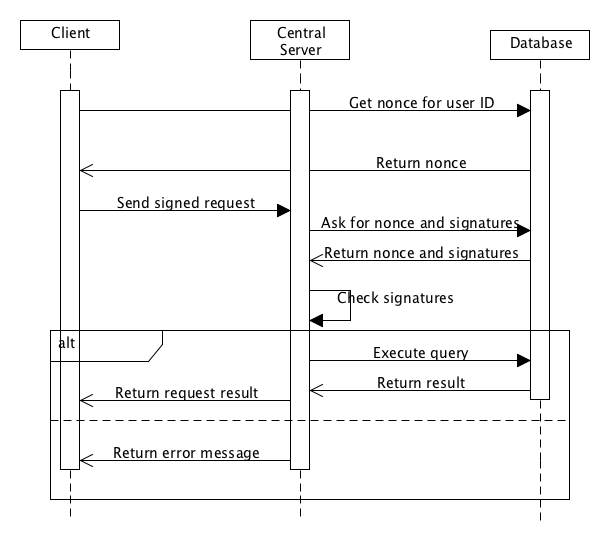
\includegraphics[width=0.8\textwidth]{database/nonce.png}
\caption{Sequence diagram of executing request with nonce signature}
\end{figure} 

\subsection{Database functions for users}
After veryfing credentials sent by user to Central Server via SSL secure channel, user, depending on its role, will be able to execute set of functions, which will serve single purpose each (e.g. creation of new prescription).

\subsubsection{Shared functions}
%Browse medicines

    \begin{longtable}{| p{6cm} | p{7.75cm} |}
    \hline
     & browse\_medicines \\ \hline
    Arguments: &  \begin{itemize}
    \item name (string, optional, default = None)
    \item type (string, optional, default = None)
	\end{itemize}        \\ \hline
    Usage: & Pharmacist sends his id and id of current patient which are signed by both of their keys. Pharmacist can see only prescriptions which are not yet realized. \\ \hline
    Result: & \begin{itemize}
    	\item medicine\_id
    	\item name
    	\item prescription requirement
    	\item medicine type
    	\item maximum dosage
    	\item unit
	\end{itemize}     \\ \hline	
    \end{longtable}

Note: Multiple records may be returned at single request.
%Browse doctors
    \begin{longtable}{| p{6cm} | p{7.75cm} |}
    \hline
     & browse\_doctors \\ \hline
    Arguments: &  \begin{itemize}
    	\item name ( string, optional, default = None)
		\item address (string, optional, default = None)
		\item license\_number (string, optional, default = None)

	\end{itemize}     \\ \hline
    Usage: & Entity using this function performs simple query which return all public data regarding registered doctors stored in DB. Arguments name, adress and license\_number narrows down result applying filters to the executed query. \\ \hline
    Result: & \begin{itemize}
    	\item doctor\_id
		\item name
		\item address
		\item license\_number
		\item certificate
		\item public\_key
	\end{itemize}     \\ \hline	
    \end{longtable}

Note: Multiple records may be returned at single request.

%Browse Pharmacies

    \begin{longtable}{| p{6cm} | p{7.75cm} |}
    \hline
     & browse\_pharmacists \\ \hline
    Arguments: &  \begin{itemize}
    	\item pharmacist\_name ( string, optional, default = None)
		\item address (string, optional, default = None)
		\item license\_number (string, optional, default = None)
		\item pharmacy\_name (string, optional, default = None)

	\end{itemize}     \\ \hline
    Usage: & Entity using this function performs simple query which return all public data regarding registered pharmacists stored in DB. Arguments name, adress and license\_number narrows down result applying filters to the executed query. \\ \hline
    Result: & \begin{itemize}
    	\item pharmacist\_id
		\item name
		\item address
		\item license\_number
		\item certificate
		\item public\_key
		\item pharmacy\_name
	\end{itemize}     \\ \hline	
    \end{longtable}
Note: Multiple records may be returned at single request.

\subsubsection{Patient functions}

%GetPatientNonce

    \begin{longtable}{| p{6cm} | p{7.75cm} |}
    \hline
     & get\_patient\_nonce \\ \hline
    Arguments: &  \begin{itemize}
    	\item patient\_id (integer, mandatory)
	\end{itemize}     \\ \hline
    Usage: & Function returns 1024 bit nonce for given patient\_id. \\ \hline
    Result: & \begin{itemize}
    	\item nonce
	\end{itemize}     \\ \hline	
			Comment: & New nonce is generated only if the last request was successfully verified.\\ \hline
    \end{longtable}


%Browse My Prescriptions History

    \begin{longtable}{| p{6cm} | p{7.75cm} |}
    \hline
     & browse\_my\_prescriptions\_history \\ \hline
    Arguments: &  \begin{itemize}
    	\item patient\_id (integer, mandatory)
		\item executed (boolean, optional, default = None)
		\item start (date, optional, default = None)
		\item end (date, optional, default = None)
		\item patient\_signature (varbinary, mandatory)
	\end{itemize}     \\ \hline
    Usage: & Patient requires history of his prescriptions. In order to get access to this kind of data, patient needs to sign his request using his secret key. Next, the signature will be veryfied by database. If signature will be acknowledged as genuine, database will return data about patient prescription history. Database provides patient the ability to filter his history by mean of time span and by the information about execution of prescriptions. \\ \hline
    Result: & \begin{itemize}
    	\item prescription\_id
    	\item doctor\_id
    	\item doctor name
    	\item doctor address
    	\item doctor license number
    	\item prescription\_owner\_id
    	\item drug id
    	\item dosage
    	\item max dosage
    	\item unit
    	\item quantity
    	\item execution
    	\item time of execution
    	\item pharmacy\_id
    	\item pharmacy\_name
    	\item pharmacy\_adress
	\end{itemize}     \\ \hline	
    \end{longtable}
Note: Multiple records may be returned at single request.

%transfer_prescription

    \begin{longtable}{| p{6cm} | p{7.75cm} |}
    \hline
     & transfer\_prescription\\ \hline
    Arguments: &  \begin{itemize}
    	\item patient\_id (integer, mandatory)
    	\item owner\_PESEL (integer, mandatory)
		\item prescription\_id (integer, mandatory)
		\item patient\_signature (varbinary, mandatory)
	\end{itemize}     \\ \hline
    Usage: & Patient changes prescription owner to another patient, therefore allowing him to buy out specific prescription. It is important note, that after changing owner of prescription, original owner is NOT able to buy out his prescription until transfer is cancelled. \\ \hline
    Result: & \begin{itemize}
    	\item new\_owner\_id
		\item "OK"

	\end{itemize}     \\ \hline	
		Comment: & Prescription in database structure has two fields indicating prescription ownership - patientID (non-changeable, indicates the patient to which the medicine was prescribed) and owner\_PESEL (patient which will may realize the prescription).
		Transfering the right will only apply if both of these fields point to same id - thus we exclude the scenario when patients can pass the prescription to yet another person. After this operation the transferring patient losses right to realize the prescription - prevention from cloning the prescription.\\ \hline
    \end{longtable}


%Cancel prescription transfer

    \begin{longtable}{| p{6cm} | p{7.75cm} |}
    \hline
     & cancel\_prescription\_transfer \\ \hline
    Arguments: &  \begin{itemize}
    	\item patient\_id (integer, mandatory)
		\item prescription\_id (integer, mandatory)
		\item patient\_signature (varbinary, mandatory)
	\end{itemize}     \\ \hline
    Usage: & Patient changes actual owner of his prescription back to the original one (the patient himself) allowing him to buy out prescription and disallowing former owner of prescription to do so. \\ \hline
    Result: & \begin{itemize}
    	\item "OK"
	\end{itemize}     \\ \hline	
		Comment: & Prescription in database structure has two fields indicating prescription ownership - patientID (non-changeable, indicates the patient to which the medicine was prescribed) and ownerID (patient which will may realize the prescription). Cancelling will only work if patientID and ownerID are different and the signature over request is verified. \\ \hline
    \end{longtable}

\subsubsection{Doctor functions}

%get_doctor_nonce

    \begin{longtable}{| p{6cm} | p{7.75cm} |}
    \hline
     & get\_doctor\_nonce \\ \hline
    Arguments: &  \begin{itemize}
    	\item doctor\_id (integer, mandatory)
	\end{itemize}     \\ \hline
    Usage: & Function returns 1024 bit nonce for given doctor\_id. \\ \hline
    Result: & \begin{itemize}
    	\item nonce
	\end{itemize}     \\ \hline	
			Comment: & New nonce is generated only if the last request was successfully verified.\\ \hline
    \end{longtable}


%create_prescription

    \begin{longtable}{| p{6cm} | p{7.75cm} |}
    \hline
     & create\_prescription \\ \hline
    Arguments: &  \begin{itemize}
    	\item doctor\_id (integer, mandatory)
		\item patient\_id (integer, mandatory)
		\item drug\_id (integer, mandatory)
		\item dosage (integer, mandatory)
		\item unit (integer, mandatory)
		\item quantity (integer, mandatory)
		\item doctor\_signature (varbinary, mandatory)
	\end{itemize}     \\ \hline
    Usage: & Doctor prescribe single medicine to the patient, describing medicine, quantity and dosage. \\ \hline
    Result: & \begin{itemize}
    	\item "OK"
	\end{itemize}     \\ \hline	
		Comment: & Database does not requires patient signature to create a prescription for him - Prescription realization will require his key (thus his smartcard) so the medicine can't be bought without his knowledge. Also the doctor can create prescription without the need of meeting the patient face to face - which is and advantage for chronically ill patients.\\ \hline
    \end{longtable}


%browse_patient_prescription_history

    \begin{longtable}{| p{6cm} | p{7.75cm} |}
    \hline
     & browse\_patient\_prescription\_history \\ \hline
    Arguments: &  \begin{itemize}
    	\item doctor\_id (integer, mandatory)
		\item patient\_id (integer, mandatory)
		\item start (date, optional, default = None)
		\item end (date, optional, default = None)
		\item bought(boolean, optional, default = None)
		\item doctor\_signature (varbinary, mandatory)
		\item patient\_signature (varbinary, optional)

	\end{itemize}     \\ \hline
    Usage: & Doctor downloads patient prescription history. Doctor (unlike pharmacist) do not needs patient signature to browse history od prescription that he has created. If he wants the full history, patients signature is needed. \\ \hline
    Result: & \begin{itemize}
    	\item prescription\_id
    	\item doctor\_id
    	\item doctor name
    	\item doctor address
    	\item doctor license number
    	\item prescription\_owner\_id
    	\item drug id
    	\item dosage
    	\item max dosage
    	\item unit
    	\item quantity
    	\item execution
    	\item time of execution
    	\item pharmacy\_id
    	\item pharmacy\_name
    	\item pharmacy\_adress
	\end{itemize}     \\ \hline
	Comment: & If the patient signature is missing, database will only return prescriptions which were created by the doctor. If the patient signature is present and can be verified, doctor will receive the full history of patient. In case of any errors on verification, the request will be canceled. \\ \hline
    \end{longtable}
Note: Multiple records may be returned at single request.

\subsubsection{Pharmacist functions}

%get_pharmacist_nonce

    \begin{longtable}{| p{6cm} | p{7.75cm} |}
    \hline
     & get\_pharmacist\_nonce \\ \hline
    Arguments: &  \begin{itemize}
    	\item pharmacist\_id (integer, mandatory)
	\end{itemize}     \\ \hline
    Usage: & Function returns 1024 bit nonce for given pharmacist\_id. \\ \hline
    Result: & \begin{itemize}
    	\item nonce
	\end{itemize}     \\ \hline	
			Comment: & New nonce is generated only if the last request was successfully verified.\\ \hline
    \end{longtable}

%prescription_realization

    \begin{longtable}{| p{6cm} | p{7.75cm} |}
    \hline
     & prescription\_realization \\ \hline
    Arguments: &  \begin{itemize}
    	\item prescription\_id (integer, mandatory)
		\item pharmacist\_id (integer, mandatory)
		\item drug\_id (integer, mandatory)
		\item unit (integer, mandatory)
		\item quantity (integer, mandatory)
		\item pharmacist\_signature (varbinary, mandatory)
		\item patient\_signature (varbinary, mandatory)

	\end{itemize}     \\ \hline
    Usage: & Pharmacist will be able to realize patient prescription by pointing right prescription by giving its id, choose proper medicine (not necessairly the same as medicine prescribed by doctor, this check will be done by database), describe how many medicine is sold.\\ \hline
    Result: & \begin{itemize}
    	\item "OK"
	\end{itemize}     \\ \hline	
	Comment: & Request has to be signed by both patient's and pharmacist's keys. If the signature is incorrect, the database will return error message and the medicine shouldn't be given away.\\ \hline
    \end{longtable}


%browse_active_prescriptions

    \begin{longtable}{| p{6cm} | p{7.75cm} |}
    \hline
     & browse\_active\_prescriptions \\ \hline
    Arguments: &  \begin{itemize}
    	\item pharmacist\_id (integer, mandatory)
		\item patient\_id (integer, mandatory)
		\item pharmacist\_signature (varbinary, mandatory)
		\item patient\_signature (varbinary, mandatory)
	\end{itemize}     \\ \hline
    Usage: & Pharmacy is able to see all active (not bought) prescriptions of current patient, which agrees to show this data to the pharmacy by signing request. \\ \hline
    Result: & \begin{itemize}
    	\item prescription\_id
    	\item doctor\_id
    	\item doctor name
    	\item doctor address
    	\item doctor license number
    	\item prescription\_owner\_id
    	\item drug id
    	\item dosage
    	\item max dosage
    	\item unit
    	\item quantity
    	\item execution
    	\item time of execution
	\end{itemize}     \\ \hline	
		Comment: & If the signatures of patient or pharmacist are incorrect, database will return an error. If there are no non-realized prescriptions, database will return empty list.\\ \hline
    \end{longtable}
Note: Multiple records may be returned at single request.

\subsection{Database schema}

\begin{figure}[h]
\begin{center}
\includegraphics[width=1.25\textwidth , angle=90]{database/databaseSchema.png}
\end{center}
\end{figure} 

\section{Central Server security standards}
\subsection{Physical Security}
\begin{itemize}
	\item Servers is protected by backup and offsite data storage. The offsite storage of backup media is in a secure backup-vendor secure facility.
	\item A facility with Uninterruptible Power Supply (UPS) supporting all servers and essential peripheral equipment (console servers, etc).
	\item A facility with a climate controlled environment separate from the building HVAC, (dedicated air conditioning with in-room temperature controls).
	\item A facility with cooling and electrical capacity that is planned and monitored for outages.
	\item Secured access to the facility with documentation listing all individuals who currently have access and monitoring/auditing of ingress/egress via staff/video/etc.
	\item Servers in the facility must require authentication for local access (i.e. consoles are not left logged in while unattended).
	\item For facilities that use access codes, the capability to quickly change the access codes if personnel changes warrant is required.  Access codes must be changed at least annually.
	\item A facility with automated fire detection and suppression systems.
\end{itemize}



\subsection{Data encryptuion}

\begin{itemize}
	\item Hard disks, on which are stored databases, will be encrypted by external program TrueCrypt. TrueCrypt encrypts whole data on hard disk in real time. 
	\item Databases will be encrypted by TDE (Transparent Data Encryption). TDE encrypts:
        \begin{itemize}
			\item Database files
			\item Database Snapshots
			\item Transaction Log File
            \item Backups
		\end{itemize}
	using DEK ( Database Encryption Key ) which is protected by certificate.
\end{itemize}

\subsection{Backup procedure}
\begin{itemize}
	\item To ensure no data loss, database is replicated in real-time to a server in another location - this location meets conditions mentioned in section 5.1.
	\item Additionally, regular backups are made every day.
	\item Backups are kept for reasonable amount of time:
        \begin{itemize}
			\item Daily backups - 1 week
			\item Weekly backups - 1 month
			\item Monthly backups - 1 year
			\item Annual backups - forever
		\end{itemize}
	\item All backups are encrypted with measures described in section 5.2.
\end{itemize}